\documentclass{article}
\usepackage[utf8]{inputenc}
\usepackage{graphicx}
\usepackage[margin=2.5cm]{geometry}
\usepackage{eso-pic}
\usepackage{hyperref}
\usepackage{wrapfig}
\usepackage{lipsum}
\usepackage{array}
\usepackage{enumitem}
\AddToShipoutPictureBG{%
    \AtPageLowerLeft{
        % \hspace{1cm}
        
\includegraphics[width=4.5cm]{img/Java-Hutts2.png}
    }
}
\title{System Requirements Specification}
\date{2017}
\def \project{Electronic ID Verification }
\begin{document}

\makeatletter
    \begin{titlepage}
        \begin{center}
            
\includegraphics[width=0.7\linewidth]{img/up.png}\\[4ex]
            {\huge \bfseries \@title }\\[2ex]
            {\LARGE \textbf{Team:} Java the Hutts}\\[2ex]
            {\LARGE \@date}\\[2ex]
            {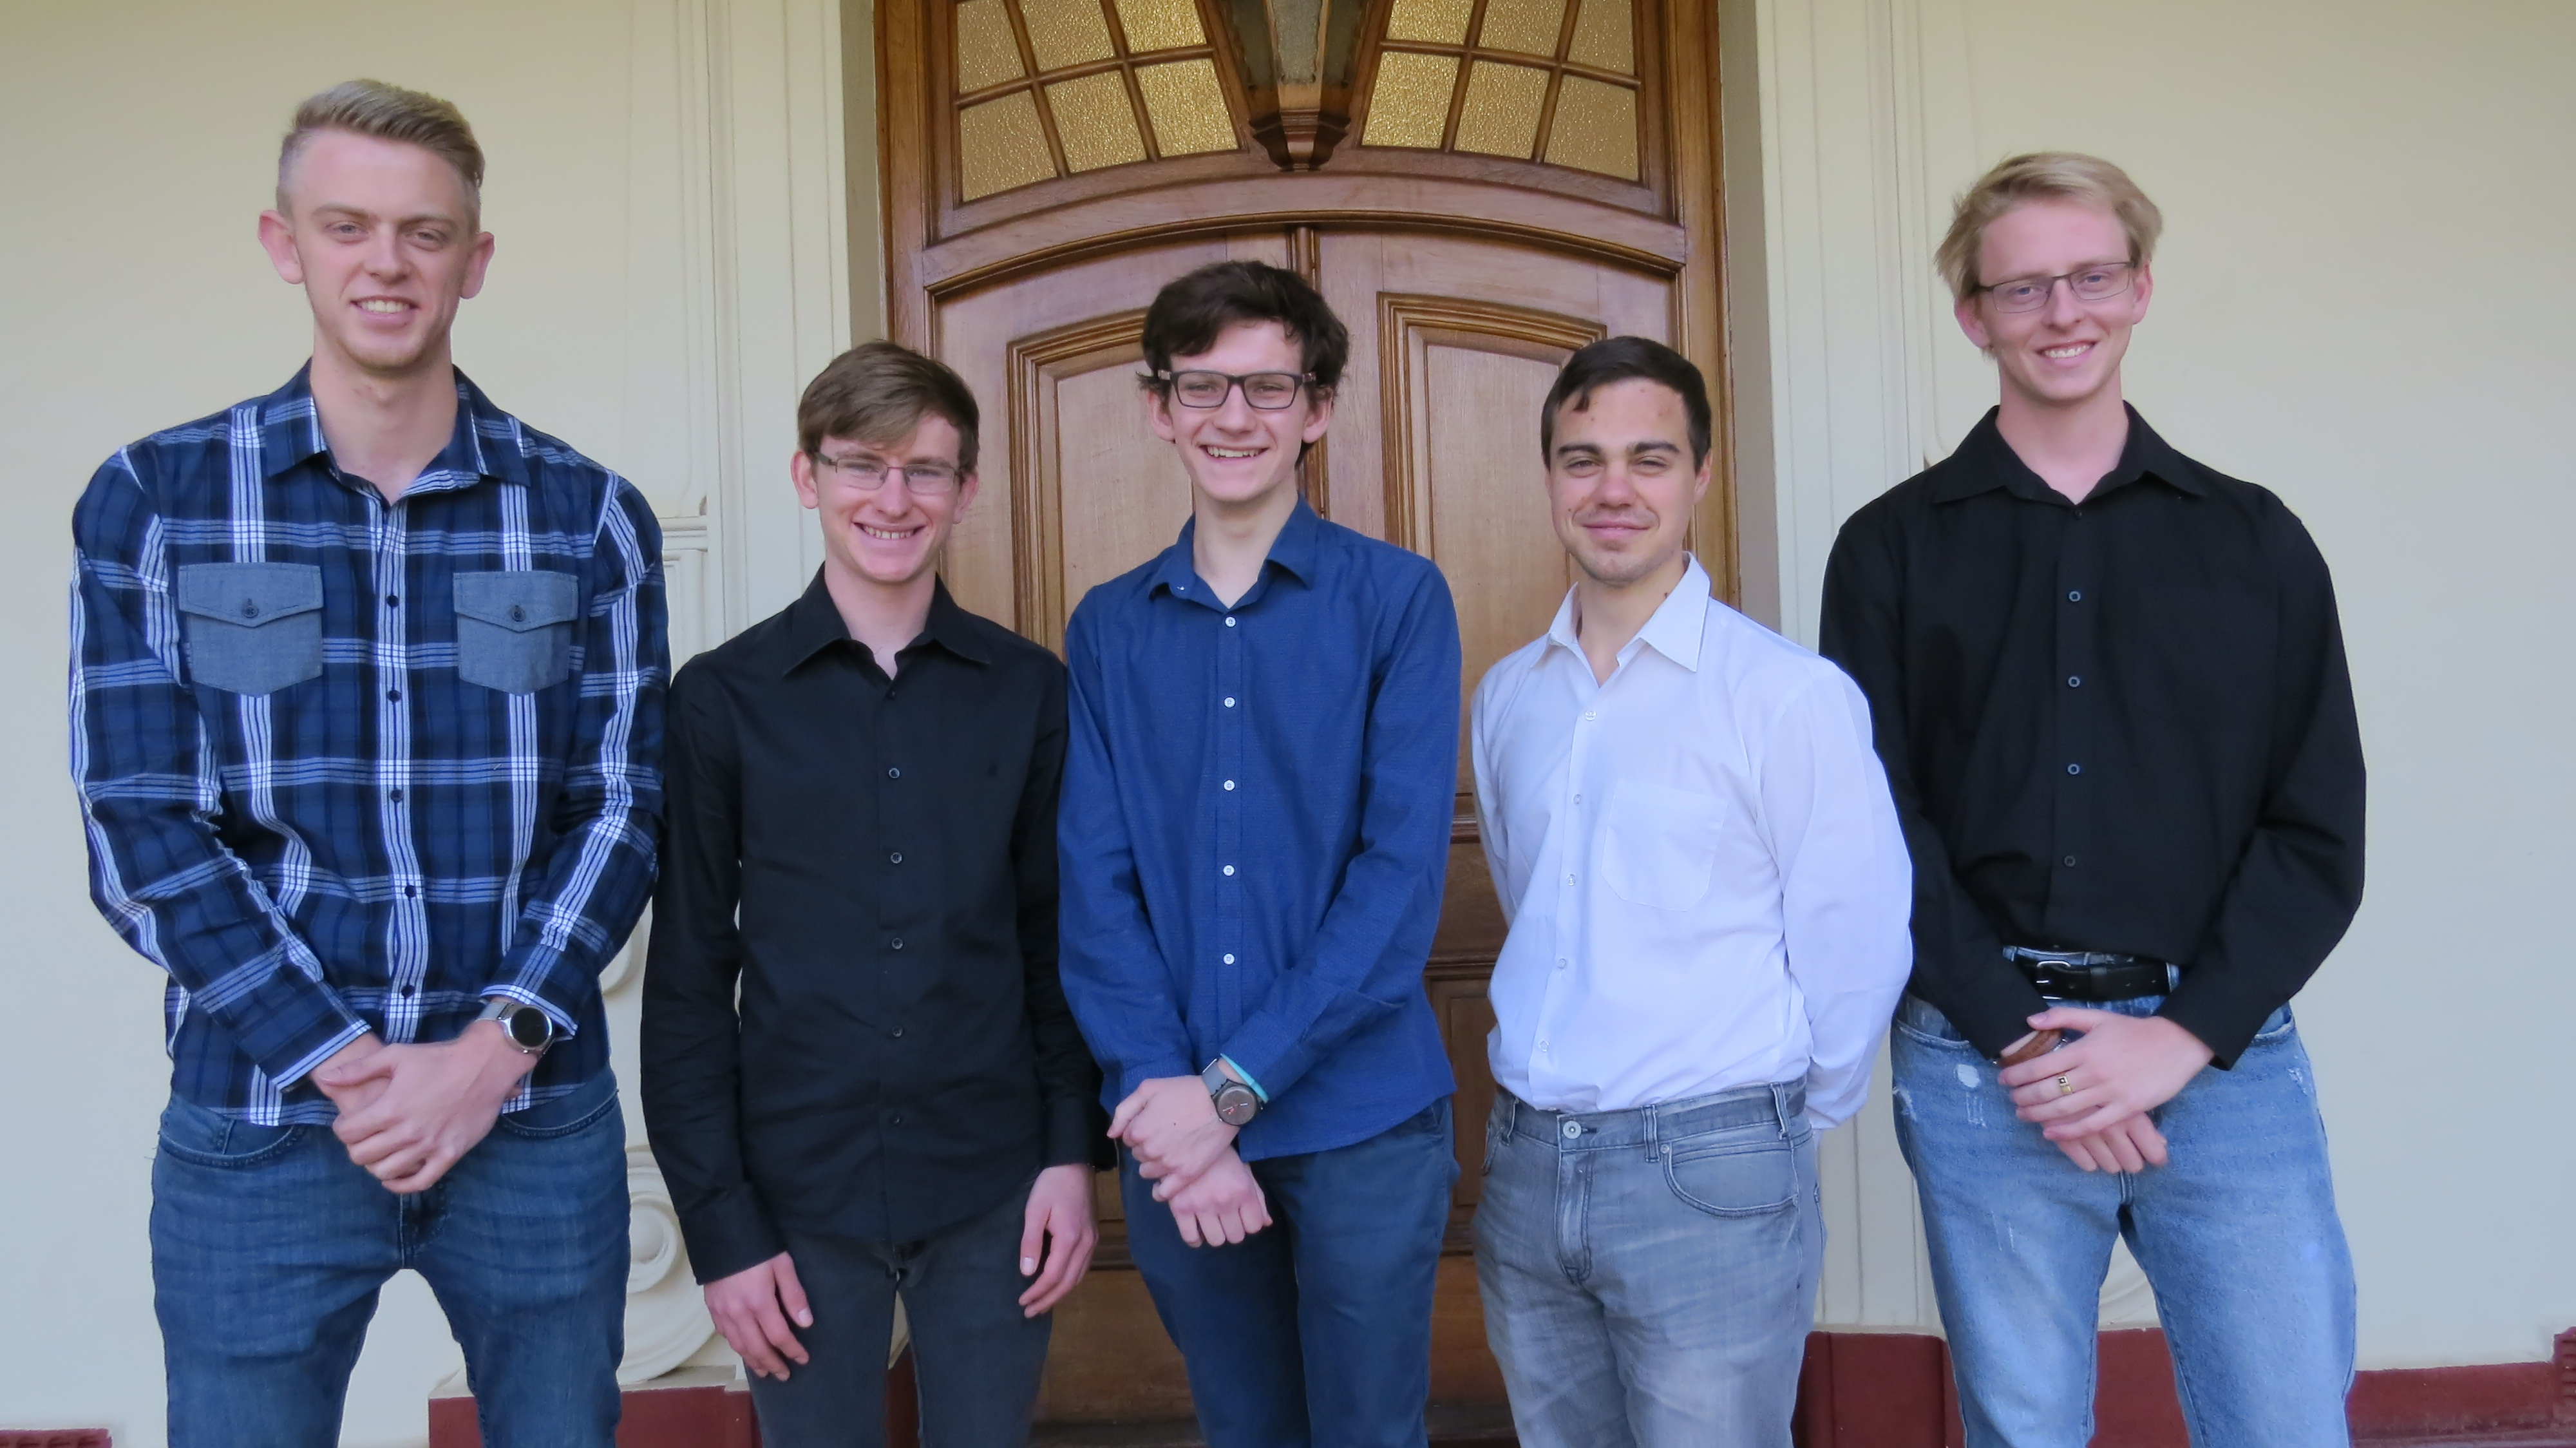
\includegraphics[width=\linewidth]{img/team_photo.jpg}}\\[2ex]
            {\large  Nicolai van Niekerk\\ \texttt{nicvaniek@gmail.com}}\\[2ex]
            {\large  Marno Hermann\\ \texttt{marno@barnton-consulting.co.za}}\\[2ex]
            {\large  Stephan Nell\\ \texttt{nellstephanj@gmail.com}}\\[2ex]
            {\large  Jan-Justin van Tonder\\ \texttt{J.vanTonder@tuks.co.za}}\\[2ex]
            {\large  Andreas Nel\\ \texttt{nel.andreas1@gmail.com}}\\[2ex]
        \end{center}
        
    \end{titlepage}
\makeatother

\cleardoublepage
\thispagestyle{empty}
\tableofcontents
\newpage

\setcounter{page}{1}
	\section{Introduction}\label{sec:intro}
		This chapter aims to give a description, as well as an overview, of the content of this document. Additionally, it will include any terms, abbreviations, acronyms and references used throughout this document.

		\subsection{Purpose}\label{subsec:purpose}
			The purpose of this document is to present the reader with a detailed description of the \project system. It will delve into the purpose and features of the system, the various interfaces of the system, the capabilities of the system, as well as the constraints under which the system must operate. The content of this document is intended for both the various stakeholders and the developers of the \project system.

		\subsection{Scope}\label{subsec:scope}
			The \project is a proposed standalone system that provides the core functionality of extracting client details from an image of some form of ID, and comparing existing client information with that of an image of some form of ID.

		\subsection{Definitions, Acronyms, and Abbreviations}\label{subsec:daa}
			\begin{table}[h!]
				\centering
				\label{tab: Table 1}
				\begin{tabular}{| m{4cm} | m{12cm} |}
					\hline
                        \textbf{Term} & \textbf{Definition}\\
					\hline
				    	OCR & Optical Character Recognition\\
				    \hline
			            ID & Identification Document\\
					
				    \hline
				        API & A set of functions and procedures that allow the creation of applications which access the features or data of an operating system, application, or other service. \\
				    \hline
				        Linux &  A Unix-like computer operating system assembled under the model of free and open-source software development and distribution\\
					\hline
					    Python & Python is a widely used high-level programming language for general-purpose programming.\\
					\hline
                    
				\end{tabular}
			\end{table}
		    
		\subsection{Overview}\label{subsec:overview}
			The remainder of this document will consist of two remaining chapters.\\

            \noindent The second chapter will address the overall description of the \project system. In addition to this, chapter two will describe the context of the \project system, its relations and the potential interfaces with other systems. This chapter will also provide a summary of the functions of the \project system as well as consider the numerous user characteristics, constraints, assumptions and dependencies relevant to the system.\\
            
            \noindent The third chapter serves the purpose of describing the software requirements of the \project system. This chapter will address the External Interface Requirements, Functional Requirements, Performance Requirements, Design Constraints, Software System Attributes and any other requirements not previously explored.\\

	\cleardoublepage

	\section{Overall Description}\label{sec:overall-description}
		This chapter aims to give an overview of the entire \project system. The system will be contextualised in order to demonstrate the basic functionality of the system as well as demonstrate how the system interacts with other systems. It will also describe the levels, or types, of users that will utilise the system and describe the functionality that is available to said user. At the end of this chapter, the constraints and assumptions for the system will be addressed.

		\subsection{Product Perspective}\label{subsec:overall-product-perspective}
		The system will be designed in the form of an API. The API will be integrated alongside the client's other software and technologies.\\
		
		 \noindent The application will focus on two main criteria. The first is that the application should be able to extract a name, surname, ID number and face, from a photo of either an ID book, ID card, driver's license or passport. The application should then take the information that was extracted and compare it to existing profile and then a percentage match score for each corresponding value should be returned.\\
		 
		  \noindent When comparing the face for a similarity percentage, the application will deal with problems like an old photo or changed facial features like a beard. By manipulating the photo with different methods to ensure that highest accuracy is ensured when matching with a photo.\\
		  
		  \noindent The second feature extracts the information from the identification photo and returns the collection of the information that the application extracted.

		\subsection{User Characteristics}\label{subsec:overall-user-characteristics}
		    The intent of the \project system is to function as an API, thus the users will require some knowledge in Python programming. The user will also require some skill and knowledge about Linux based operating systems like Ubuntu since development in Linux is a requirement of the client.

		\subsection{Constraints}\label{subsec:overall-constraints}
			Only a valid South African ID book, South African ID card, South African Driver license or South African Passport can be used with the application.\\
			
			\noindent People's facial features could change or the photo provided could be very old, or the individual in the photo could be standing skew and not providing a full frontal facial image.

		\subsection{Assumptions and Dependencies}\label{subsec:overall-asusmptions-and-dependencies}
		\begin{itemize}
		    \item It is assumed that enough resources will be provided to test multiple ID cards, ID books, driver's licenses or passports.
		    \item It is assumed that a clear and well-lit photo will always be provided.
		    \item It is assumed that all identification documentation follows the format of documentation issued in South Africa.
		\end{itemize}
			

	\cleardoublepage

	\section{Specific Requirements}\label{sec:specific-requirements}
		This chapter addresses all the functional requirements of the \project system. It gives a detailed description of the system and all its features.

		\subsection{External Interface Requirements}\label{subsec:specific-external}
		\subsubsection{User-interfaces}
		The system will be implemented as an API that will be called from within Quant Solutions' web framework. As a result there are no user-interface requirements.
		\subsubsection{Hardware Interfaces}
		No extra hardware interface is needed, since the application is designed as a API and is completely detached from any hardware requirements.
		\subsubsection{Software Interfaces}
		Since the system will be implemented as an API, it will interface with the existing systems of Quant Solutions. 
		\subsubsection{Communication Interfaces}
		Communication is an important aspect of an API to function correctly. The application must be able to pass the correct information to any system that makes use of the application functionality. It is also important that descriptive responses are provided in case of an error, or if the need arises to provide extra information.\\
			

		\subsection{Functional Requirements}\label{subsec:specific-functional}
		This section describes the functional requirements of the system. The requirements are derived from the specific use cases that are modelled using use case diagrams. Non-trivial use cases are also further elaborated using Actor-System interaction diagrams.
		
		\begin{enumerate}
		    \item \textbf{FR-01:} The system must be able to accept the relevant input data and a(n) ID/Passport/License photo in a specified format.
		    \item \textbf{FR-02:} The system must be able to extract text from the provided image.
		    \item \textbf{FR-03:} The system must be able to extract the photo from the image.
		    \item \textbf{FR-04:} The system must be able to detect a face from the extracted image.
		    \item \textbf{FR-05:} The system must be able to age the detected face to a specified date.
		    \item \textbf{FR-06:} The system must be able to align a face for better matching.
		    \item \textbf{FR-07:} The system must be able to compare the extracted text with provided data.
		    \item \textbf{FR-08:} The system must be able to compare two faces after image processing.
		    \item \textbf{FR-09:} The system must be able to give a percentage match on the validated data.
		    \item \textbf{FR-10:} The system must be able to visually show the differences in images.
		    \item \textbf{FR-11:} The system must be able to perform extraction on a South African ID book.
		    \item \textbf{FR-12:} The system must be able to perform extraction on a South African ID card.
		    \item \textbf{FR-13:} The system must be able to perform extraction on a South African driver's license.
		    \item \textbf{FR-14:} The system must be able to perform extraction on a South African passport.
		    \item \textbf{FR-15:} The system must allow a user to specify a matching accuracy threshold.
		    \item \textbf{FR-16:} The system must be able to remove beards and/or piercings from the detected face.
		    
		\end{enumerate}
		
		
		\subsection{Performance Requirements}\label{subsec:specific-performance}
		\begin{itemize}
		    \item The application should be versatile enough to handle any future enhancement, like supporting a wider variety of identification materials.
		    \item Any internal errors and exceptions should be handle by the system itself.
		    \item The system should function in real time. All OCR request should be handled in under 5 seconds.
		    \item Any request with regards to facial comparisons and image optimisation should be handled in under 10 seconds.
		    \item The system should be able to handle a high amount of concurrent requests within an acceptable timeframe.
		\end{itemize}

		\subsection{Design Constraints}\label{subsec:specific-constraints}
		\begin{itemize}
		    \item The system will be implemented using Python 3.5 in order to ensure compatibility between the API and the Quant Solutions system.
		\end{itemize}			

		\subsection{Software System Attributes}\label{subsec:specific-software}
		This section describes all quality related requirements
		\subsubsection{Reliability}
		\begin{enumerate}
		    \item The system should not fail when given a clear, well-lit photo of the identification document.
		    \item The system should always give a percentage match above the specfied threshold if the faces are the same.
		    \item Error handling should be implemented and the application should be able to handle all errors in a graceful manner by making use of helpful and descriptive error messages.
		\end{enumerate}
		\subsubsection{Security}
		\begin{enumerate}
		    \item All incoming and outgoing data will be encrypted due to the sensitive nature of the data collected.
		\end{enumerate}
		\subsubsection{Availability}

		\subsection{Other Requirements}\label{subsec:specific-other}
		\begin{itemize}
            \item Documentation should be of such a standard that anyone can easily implement the application when needed.
            \item The system should indicate that images match only if the images match with an accuracy of at least 75\%.
		\end{itemize}

	\cleardoublepage

\end{document}
